
\section{Empirical Results}\label{sec:experiments}

We use COVID-19 hospitalization data, which can be downloaded from \href{https://forecast-eval.s3.us-east-2.amazonaws.com/hospitalizations.zip}{this link}. 
The observed hospitalizations are provided by the U.S. Department of Health \& Human Services and correspond to the total number of adult and pediatric COVID-19 admissions. 
The hospitalization forecasts are obtained from the \href{https://github.com/reichlab/covid19-forecast-hub/}{COVID-19 Forecast Hub GitHub repository} \cite{cramer2022covidhub}.

The dataset contains state-level hospitalization forecasts (covering the 50 states and the District of Columbia) as well as the U.S. aggregate (hereafter, US-agg), totaling 52 series for $N=23$ quantile levels at $h$ weeks ahead, for horizons $h \in \{1,2,3,4\}$. 
We restrict our attention to forecasts from $B=18$ forecasting teams (referred to as \emph{base forecasters}) and two ensemble models: COVIDhub-4\_week\_ensemble (COVIDhub-Ens) and JHUAPL-SLPHospEns (JHUAPL-SLPEns), both constructed as ensembles of base forecasters. 
We consider $T=127$ weeks of data from December 2020 to June 2023. 
Additional details are deferred to Appendix~\ref{appsubsec:experiment_details}.

We run Algorithm~\ref{alg:omni-twoplayer_online_multi_q}, which we refer to as \textit{our algorithm} hereafter, on the $B=18$ base forecasters. We compare its predictions with those from the two ensemble models, as well as with Algorithm~\ref{alg:wql_hedge}, which we refer to as \textit{Hedge-QL} hereafter.

\paragraph{Metrics}
We evaluate performance using two metrics: the omniprediction error and the quantile loss. 
Given base forecasters $\{\hat{f}_b^n\}_{b=1}^B$ that provide $\{\tau_n\}_{n=1}^N$-level quantile forecasts $\{\hat{f}_b^n(t)\}_{n=1}^N$, the (cumulative) omniprediction error at time $t$ for a forecast $\{P_t^n\}_{n=1}^N$ is defined as
\begin{align}\label{eq:omni_error_def}
\sup_{S \in \cs,\, b \in [B]} \frac{1}{t} \sum_{n=1}^N \sum_{s=1}^t \E_{p \sim P_s^n} [S(p, Y_s)] - S(\hat{f}_b^n(s), Y_s).
\end{align}

The (cumulative) quantile loss is defined as
\[
\frac{1}{Y_{\text{max}}}\sum_{s=1}^t \sum_{n=1}^N \E_{p \sim P_s^n} [\rho_{\tau_n}(Y_s - p)],
\]
where $\rho_{\tau}$ is the pinball loss and $Y_{\text{max}}$ is the maximum value of the ground truth in each (horizon, region) dataset. 
We also consider the instantaneous quantile loss at time $t$: $\sum_{n=1}^N \E_{p \sim P_t^n} [\rho_{\tau_n}(Y_t - p)] / Y_t$

\paragraph{Discretization}
As introduced in Section~\ref{subsec:discretization}, we discretize both the predictions and the ground truth into a finite set of values. 
We use grid spacings from $\{2,5,10,20,50,100,500\}$ depending on the range of forecast values. 
This results in more than $500$ grid points for all $208 = 4 \times 52$ datasets, and more than $1{,}000$ grid points for over $150$ datasets. 
Additional details are provided in Appendix~\ref{appsubsec:experiment_details}.

\paragraph{Learning rates}
Our algorithm and Hedge-QL involve learning rates as hyperparameters. 
Rather than tuning these explicitly, we evaluate each algorithm over a range of learning rates, report the best performance for each metric, and provide a sensitivity analysis. 
For each metric, we select the best-performing instance in hindsight; in plots and legends, these are denoted by \textit{*Our algorithm} and \textit{*Hedge-QL}. 
For some plots, we also report results using a fixed learning rate.

When referring to our algorithm with learning rate $c$, the actual learning rate is $c \sqrt{\log (mNB) / T}$. 
For Hedge-QL, the learning rate is $c \sqrt{\log B / T} / Y_{\text{max}}$. 
We use $c=\{10^{i/4} \mid i=-12,\ldots,5\}$ for our algorithm and $c=\{10^{i/4} \mid i=-12,\ldots,16\}$ for Hedge-QL.


%%%%%%%%%%%%%%%%%%%%%%%%%%%%%%%%%%%%
% SUBSECTION
%%%%%%%%%%%%%%%%%%%%%%%%%%%%%%%%%%%%
\subsection{Forecast behavior and qualitative comparison}

\begin{figure}[htbp]
  \centering
  \begin{subfigure}{0.98\textwidth}
      \centering
      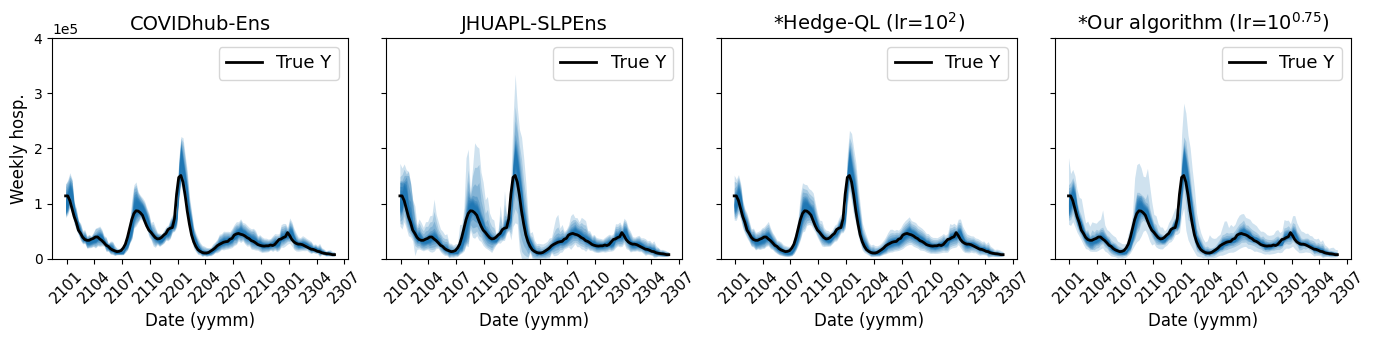
\includegraphics[width=\textwidth]{../fig/Quantile_estimates_US_1wk.png}
      \caption{$1$-week-ahead prediction.}
      \label{fig:quantile_estimates_us_1wk}
  \end{subfigure}

  \vspace{0.5em}

  \begin{subfigure}{0.98\textwidth}
      \centering
      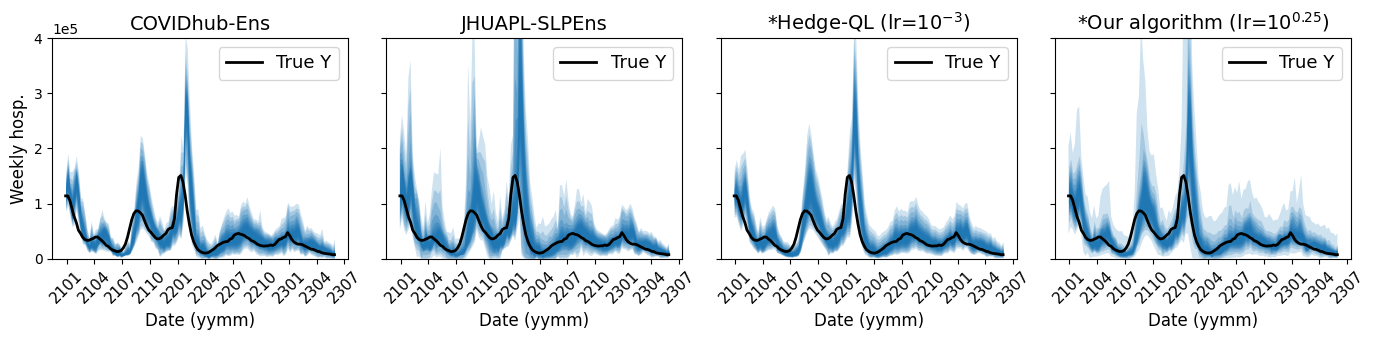
\includegraphics[width=\textwidth]{../fig/Quantile_estimates_US_4wk.png}
      \caption{$4$-week-ahead prediction.}
      \label{fig:quantile_estimates_us_4wk}
  \end{subfigure}

  \caption{
  Quantile forecasts for US-agg weekly COVID-19 hospitalizations at $1$-week-ahead and $4$-week-ahead horizons. The learning rate for \textit{*Hedge-QL} and \textit{*Our algorithm} is selected to achieve the best omniprediction error at the last time step $T$. The black curve shows the observed hospitalizations. The blue shaded regions show nested quantile prediction bands: darker regions correspond to more central quantile intervals, while lighter regions correspond to wider intervals.
  }
  \label{fig:quantile_estimates_us}
\end{figure}

Figure~\ref{fig:quantile_estimates_us} compares quantile forecasts for US-agg hospitalizations. 
COVIDhub-Ens is constructed as a weighted average of quantile estimates, whereas JHUAPL-SLPEns first constructs predictive distributions and then averages the resulting CDFs \cite{jhuapl_slphospens}. 
Hedge-QL also aggregates quantile estimates via weighted averaging. 
It is well-known that averaging quantile forecasts produces sharper intervals than averaging predictive distributions~\cite{lichtendahl2013qorcdf}.

Consistent with this, COVIDhub-Ens and \textit{*Hedge-QL} produce relatively sharp prediction bands, whereas JHUAPL-SLPEns yields wider intervals. 
Interestingly, although our algorithm only uses quantile forecasts, it produces intervals that are slightly wider than those of COVIDhub-Ens and \textit{*Hedge-QL}, yet noticeably sharper than JHUAPL-SLPEns, while still closely tracking the observed trajectory.
\bigskip

\begin{figure}[htbp]
  \centering
  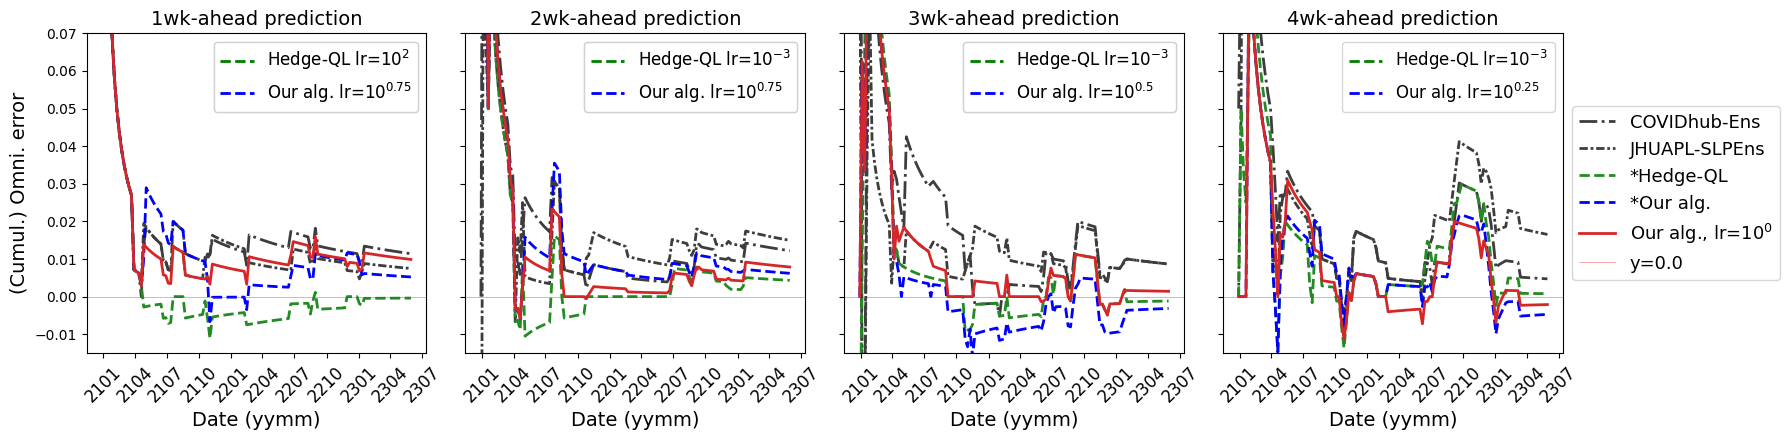
\includegraphics[width=\textwidth]{../fig/Omni_error_over_time.png}
  \caption{
  Cumulative omniprediction error \eqref{eq:omni_error_def} over time for $1$- to $4$-week-ahead forecasting horizons for US-agg. For \textit{*our algorithm} and \textit{*Hedge-QL}, the legend in each panel shows the learning rate that attains the best performance. Lower values indicate better performance.}
  \label{fig:omni_error_over_time}
\end{figure}

Figure~\ref{fig:omni_error_over_time} reports cumulative omniprediction error over time. 
As the forecasting horizon increases, the task becomes more challenging, and the advantage of \textit{*our algorithm} becomes more significant. 
In particular, for $3$- and $4$-week-ahead predictions, \textit{*our algorithm} consistently outperforms competing methods. 
Even with a fixed learning rate $c=1.0$, which minimizes the upper bound of omniprediction error in Theorem \ref{thm:omni-twoplayer_online_multi_q}, it outperforms both ensemble baselines for $2$--$4$ week horizons and outperforms \textit{*Hedge-QL} at the $4$-week horizon.



%%%%%%%%%%%%%%%%%%%%%%%%%%%%%%%%%%%%
% SUBSECTION
%%%%%%%%%%%%%%%%%%%%%%%%%%%%%%%%%%%%
\subsection{Quantitative performance across horizons and locations}

Figure~\ref{fig:error_diff_density} shows that the advantage of \textit{*our algorithm} over competing methods extends beyond the US-agg results to the state level. Across most state-level series, \textit{*our algorithm} achieves lower omniprediction error and quantile loss than two ensemble models. This improvement becomes more noticeable for longer forecasting horizons: as the horizon increases, the distributions shift further to the right, indicating larger performance gains.
Compared to \textit{*Hedge-QL}, the gains are smaller but still consistent.
\bigskip

\begin{figure}[htbp]
  \centering
  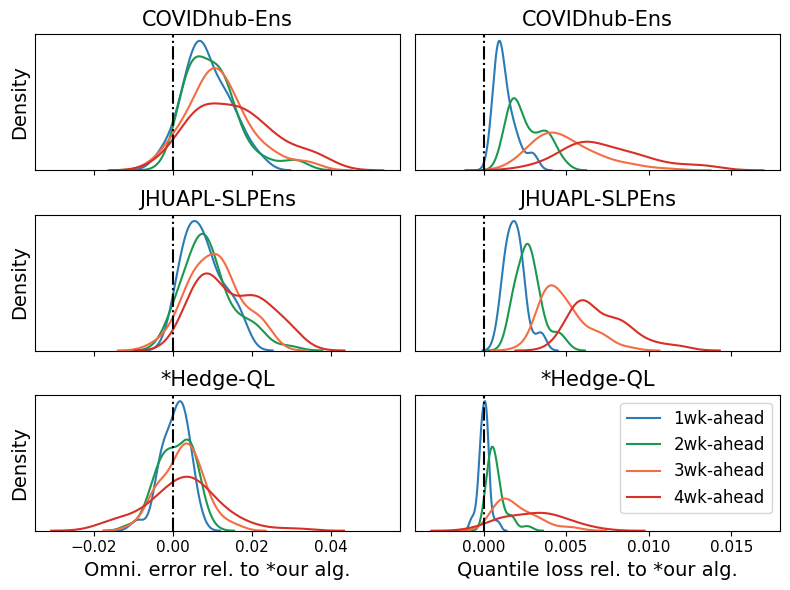
\includegraphics[width=0.6\textwidth]{../fig/Error_diff_density.png}
  \caption{
  State-level comparison of performance relative to \textit{*our algorithm}. Each row corresponds to each competing method. The left column shows differences in cumulative omniprediction error \eqref{eq:omni_error_def}, and the right column shows differences in cumulative quantile loss, computed as competitor minus \textit{*our algorithm}. Each curve shows a kernel density estimate of these differences across the $51$ state-level series for a given forecasting horizon. Values to the right of zero indicate better performance of \textit{*our algorithm}; the vertical dash-dotted line marks zero.
  }
  \label{fig:error_diff_density}
\end{figure}

\begin{figure}[htbp]
  \centering
  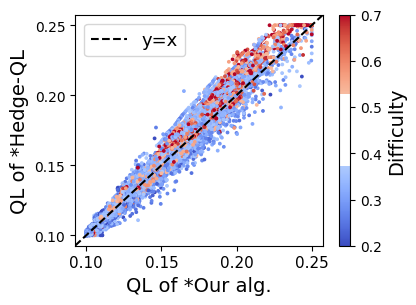
\includegraphics[width=0.55\textwidth]{../fig/Difficulty_plot.png}
  \caption{
  Comparison of instantaneous quantile loss between \textit{*our algorithm} (x-axis) and \textit{*Hedge-QL} (y-axis). Each point corresponds to a (horizon, location, time) tuple. %, for a total of $4 \times 51 \times 127 = 25{,}908$ points. 
  Color represents task difficulty, defined as \eqref{eq:difficulty_def} and clipped to the range $[0.2, 0.7]$, with red indicating more difficult instances and blue indicating easier ones.
  The dashed line denotes $y=x$, and points above the line indicate better performance of \textit{*our algorithm}. 
  }
  \label{fig:ql_scatter_difficulty}
\end{figure}

Consistent with the trends observed above, Figure~\ref{fig:ql_scatter_difficulty} shows that \textit{*our algorithm} performs particularly well on more difficult instances. The color represents the difficulty of prediction at (horizon, location, time) tuple, measured by the average pinball loss of base forecasters, which is calculated as follows:
\begin{align}\label{eq:difficulty_def}
\frac{1}{Y_t} \frac{1}{BN} \sum_{n=1}^N \sum_{b=1}^B \rho_{\tau_n}(Y_t - f_b(t)).
\end{align}
In particular, the darker (red) points are predominantly located above the $y=x$ line, indicating that \textit{*our algorithm} achieves lower quantile loss than \textit{*Hedge-QL} on harder prediction tasks.



%%%%%%%%%%%%%%%%%%%%%%%%%%%%%%%%%%%%
% SUBSECTION
%%%%%%%%%%%%%%%%%%%%%%%%%%%%%%%%%%%%
\subsection{Sensitivity Analysis}

\begin{figure}[htbp]
  \centering
  \begin{subfigure}{0.98\textwidth}
      \centering
      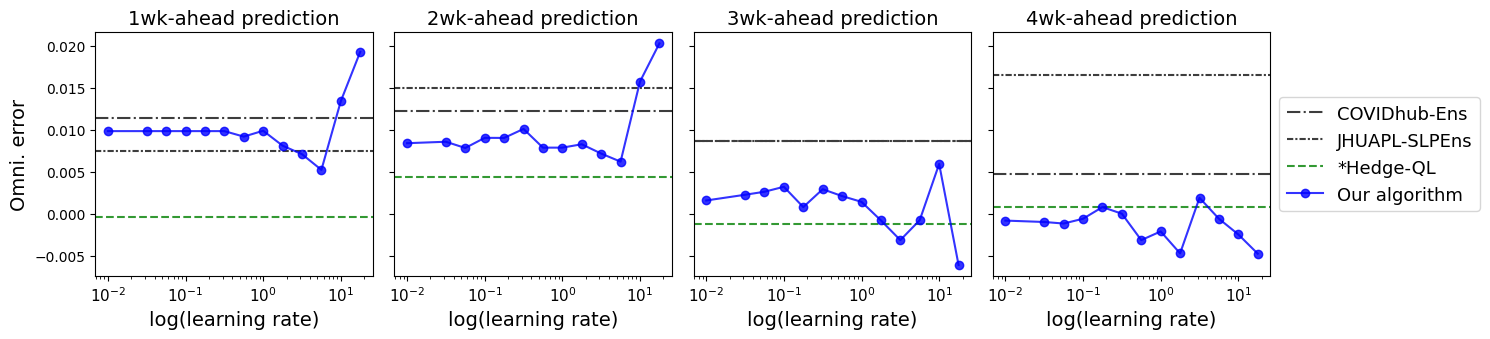
\includegraphics[width=\textwidth]{../fig/Sensitivity_omni.png}
      \caption{(Cumulative) Omniprediction error at last time step $T$ (US-agg).}
      \label{fig:sensitivity_omni}
  \end{subfigure}

  \vspace{0.5em}

  \begin{subfigure}{0.98\textwidth}
      \centering
      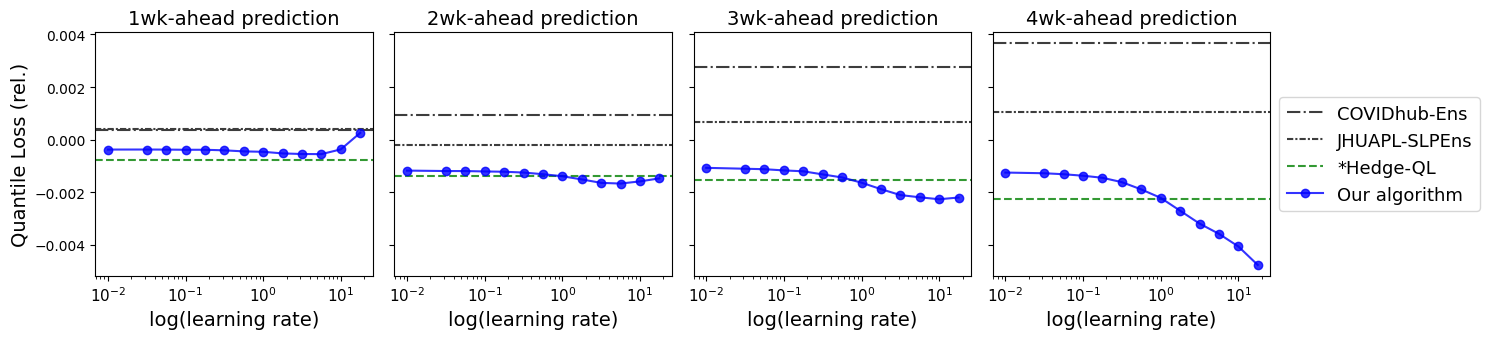
\includegraphics[width=\textwidth]{../fig/Sensitivity_QL.png}
      \caption{(Cumulative) Quantile loss at last time step $T$ (US-agg).}
      \label{fig:sensitivity_ql}
  \end{subfigure}

  \caption{
    Sensitivity of \textit{our algorithm} to the learning rate. 
    Each panel shows the performance of \textit{our algorithm} as a function of the learning rate (blue curve), while horizontal lines indicate the performance of the competing methods. 
    The bottom plot shows the quantile loss relative to that of the best base forecaster. 
    Lower values indicate better performance.
  }
  \label{fig:sensitivity}
\end{figure}


In this subsection, we show how the performance of \textit{our algorithm} varies with the learning rate. Figure~\ref{fig:sensitivity} shows the performance of \textit{our algorithm} as a function of the learning rate for $1$- to $4$-week-ahead horizons for US-agg data.
Across most horizons and learning rates, \textit{our algorithm} outperforms the two ensemble models. 
For the $4$-week-ahead horizon, it achieves lower omniprediction error than \textit{*Hedge-QL} for nearly all learning rate choices. 
We also observer that quantile loss varies more smoothly with respect to the learning rate than omniprediction error. Although the two metrics exhibit broadly similar trends, they do not coincide exactly, indicating a trade-off between the two criteria.




\begin{figure}[htbp]
  \centering
  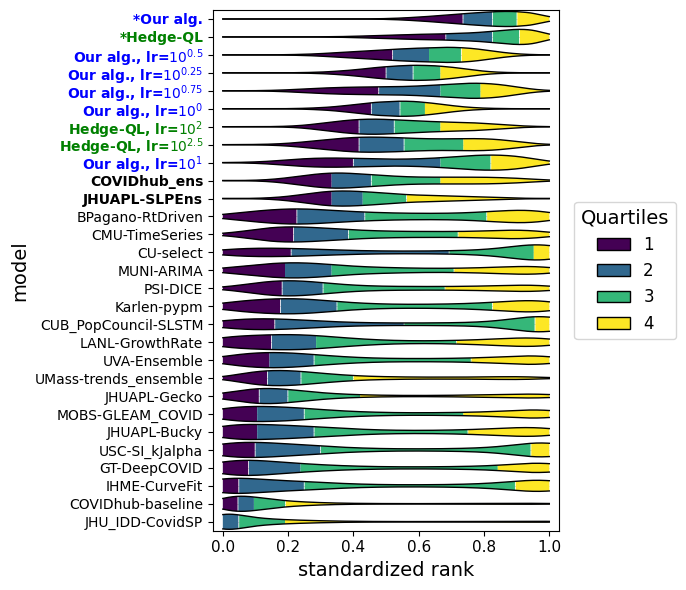
\includegraphics[width=0.8\textwidth]{../fig/QL_std_rank.png}
  \caption{
    Distribution of standardized ranks of instantaneous quantile loss across all (horizon, location, time) tuples for the $51$ state-level series. 
    For each tuple, we rank the available forecasts by quantile loss and normalize the ranks to $[0,1]$. 
    The colored segments represent the empirical distribution of ranks grouped into quartiles. 
    The visualization design is adapted from \cite{cramer2022violinplot}.
    }
  
  \label{fig:rank_distribution}
\end{figure}


Figure~\ref{fig:rank_distribution} summarizes performance of all algorithms including $18$ base forecasters using standardized ranks. Models are ordered by their first-quartile performance, with higher placement indicating better performance. 
Besides \textit{*our algorithm} and \textit{*Hedge-QL}, multiple instances of our algorithm with a fixed learning rate is ranked higher than the two ensemble models and all base forecasters. 
The first quartile of standardized ranks of all of our algorithm is higher than two ensemble models. The third quartile of our algorithm instances are comparable to or higher than those of two ensemble models. This implies that our algorithm, for a wide range of learning rates, can be viewed as better and more robust model compared to two ensemble models.